\documentclass[]{article}

%opening
\Huge\title{STAT 4352 - Mathematical Statistics Notes}
\Large\author{JaimeGoB}
\usepackage[margin=0.5in]{geometry}
\usepackage{physics}
\usepackage{amsmath}
\usepackage{centernot}
\usepackage{soul}
\usepackage{graphicx}
\graphicspath{ {../documentation/} }
\setul{}{1pt}

\begin{document}

\maketitle

\newpage
\Huge\section{Chapter 11 - Interval Estimation}
\Large\textbf{Point Estimators}
\newline $\theta$ is a unknown parameter (feature of a population)
\begin{itemize}
	\item Ex: population mean $\mu$
	\item \textbf{Fixed.} \newline
\end{itemize}
$\hat\theta$ is a point estimator of $\theta$ (it is a numerical value) 
\begin{itemize}
	\item Ex: sample mean $\bar{x}$
	\item \textbf{Varies from sample to sample.}
	\item No guarantee of \textul{accuracy}
	\item Must be \textit{supplemented by} Var($\theta$)
	\newline\Large\rule{1.3cm}{0pt} Standard Error SE($\hat\theta$) measures how much $\hat\theta$ varies from sample to sample.
	\newline\Large\rule{1.3cm}{0pt} small SE $\implies$ low variance thus a more reliable estimate of $\theta$ \newline
\end{itemize}
\Large\textbf{Interval Estimators} 
\newline
\newline\Large\textbf{Def: Interval Estimate}
\newline Provides a range of values that best describe the population.
\newline Let L = L(x) be the Lower Limit
\newline\Large\rule{0.68cm}{0pt} U = U(x) be the Upper Limit
\newline Both L,U are Random Variables because they are functions of sample data.
\newline
\newline\Large\textbf{Def: Confidence Level / Confidence Coefficient}
\newline Is the probability that the \textbf{interval estimate} will include population parameter $\theta$.
\begin{itemize}
	\item Sample means will follow the \textul{normal probability distribution} for large sample sizes (n $\ge$ 30)
	\item For small sample  forces us to use the \textul{t-distribution} probability distribution(n $<$ 30)
	\item \textul{A confidence level of 95$\%$} implies that \textbf{95$\%$ of all samples would give an interval that includes $\theta$, and only 5$\%$of all samples would yield an erroneous interval.}
	\item \textul{The most frequently used confidence levels are 90$\%$, 95$\%$, and 99$\%$ with corresponding Z-scores 1.645, 1.96, 2.576.}
	\item The higher the confidence level, the more strongly we believe that the value of the parameter lies within the interval.
\end{itemize}
\Large\textbf{Def: Confidence Interval}
\newline Gives plausible values for the parameter $\theta$ being estimated where degree of plausibility specified by a confidence level.
\newline
\newline To construct an interval estimator of unknown parameter $\theta$. We must find two statistics \textbf{L} and \textbf{U} such that:
 \[  P \{\textbf{L} \le \theta \le \textbf{U}  \}  = 1 - \alpha  \] 
\begin{itemize}
	\item $P \{\textbf{L} \le \theta \le \textbf{U} \}$ \textbf{Coverage Probability}, in repeated sampling, what percent of samples or Confident Intervals capture true $\theta$.
	\item 100(1- $\alpha$) \textbf{Confidence Interval }- for unknown fixed parameter $\theta$.
	\item L,U - \textbf{Lower and Upper Bounds} - RVs because they are functions of sample data. Vary from sample to sample.
	\item 1-$\alpha$ \textbf{Confidence Level} (Probability) estimate will include population parameter $\theta$.
	\item $\alpha$ \textbf{Level of Significance} Percent chance Confidence Interval will not contain population parameter $\theta$.
\end{itemize}
\Large\textbf{Def: Coverage Probability}
\newline $P \{\textbf{L} \le \theta \le \textbf{U} \}$ Gives what $\%$ of samples or Confidence Intervals capture true $\theta$.
\newline
\newline Ex: Coverage Probability = 95$\%$
\newline\Large\rule{1.3cm}{0pt} Will capture $\theta$, 95$\%$ of the time.
\newline\Large\rule{1.3cm}{0pt} Will NOT capture $\theta$, 5$\%$ of the time.
\newline
\newline\Large\textbf{Properties of Confidence Intervals}
\begin{itemize}
	\item Confidence Intervals are not unique.
	\item Desirable to have E[Length of CI] to be small.
	\item A one-sided 100(1-$\alpha$) lower-confidence interval on $\theta$:  L = -$\infty  \implies P\{ L \le \theta \} = 1-\alpha$
	\item A one-sided 100(1-$\alpha$) upper-confidence interval on $\theta$: $U = \infty  \implies P\{ \theta \le U \} = 1-\alpha$
	\item If L,U are both finite, then we have a two sided interval.
\end{itemize}
\Large\textbf{Correctly Interpreting Confidence Intervals}
\newline \textbf{Not Correct}
\newline There is 90$\%$ probability that the true population mean is within the interval.
\newline \textbf{Correct}
\newline There is a 90$\%$ probability that \textul{any given Confidence Interval from a random sample} will contain the true population mean.
\newline
\newline
\Large\textbf{Theorem 11.1: Confidence Interval on the Mean of a Normal Distribution with known Variance}
\newline Let X be normal random variable with:
\newline\Large\rule{1.3cm}{0pt} Unknown mean $\mu$
\newline\Large\rule{1.3cm}{0pt} Known variance $\sigma ^2$
\newline Suppose a random sample n, ($X_1, X_2,...,X_n$) is taken.
\newline A 100(1-$\alpha$)$\%$ confidence interval on $\mu$ can be obtained by considering sampling distribution of the sample mean $\bar{X}$.
\newline
\newline\Large\rule{1.3cm}{0pt}\textbf{Central Limit Theorem:} 
\newline\Large\rule{1.3cm}{0pt} E($\bar{X}$) = $\mu$ and SD($\bar{X}$) = $\dfrac{\sigma}{\sqrt{n}}$, so $\bar{X} \sim \mathcal{N}(\mu, \dfrac{\sigma ^2}{ n })  $ as n$\to \infty$
\newline
\newline \Large\rule{1.3cm}{0pt} Let Z = Standardizing $\bar{X}$, Z will follow a Standard Normal Distribution
\newline 
\newline\Large\rule{1.3cm}{0pt} Let Z = $\dfrac{\bar{X} - \mu}{\sigma \\/ \sqrt{n} } \sim \mathcal{N}(0, 1) $
\newline 
\newline We can see from the image to the \textul{left:} \textbf{Distribution of Z} and the image to the \textul{right:} \textbf{Confidence Interval of 95$\%$}
\newline
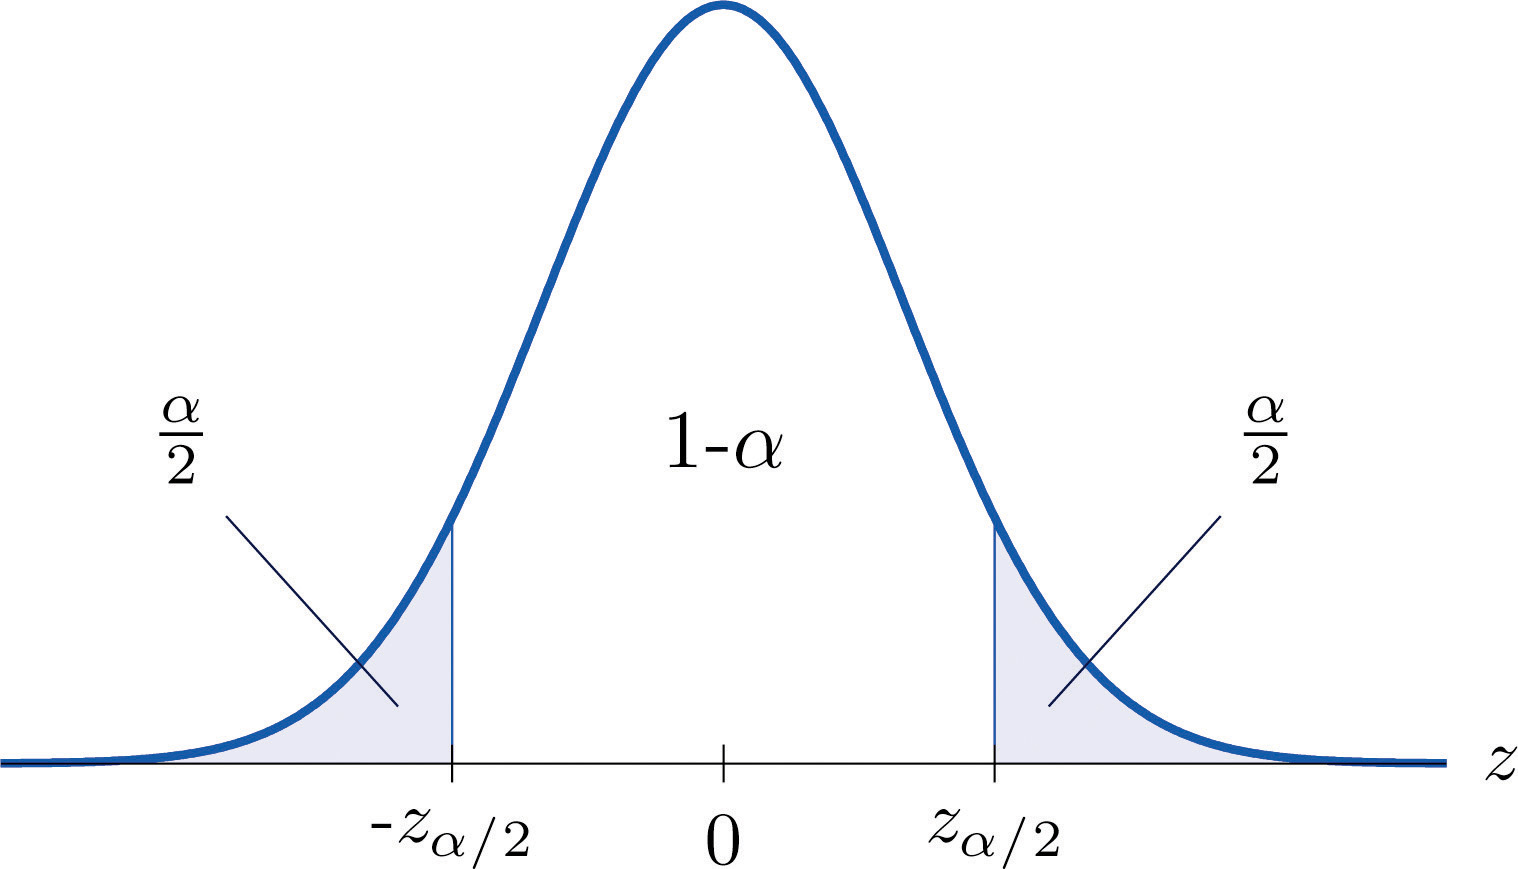
\includegraphics[scale=0.7]{distribution_of_Z}
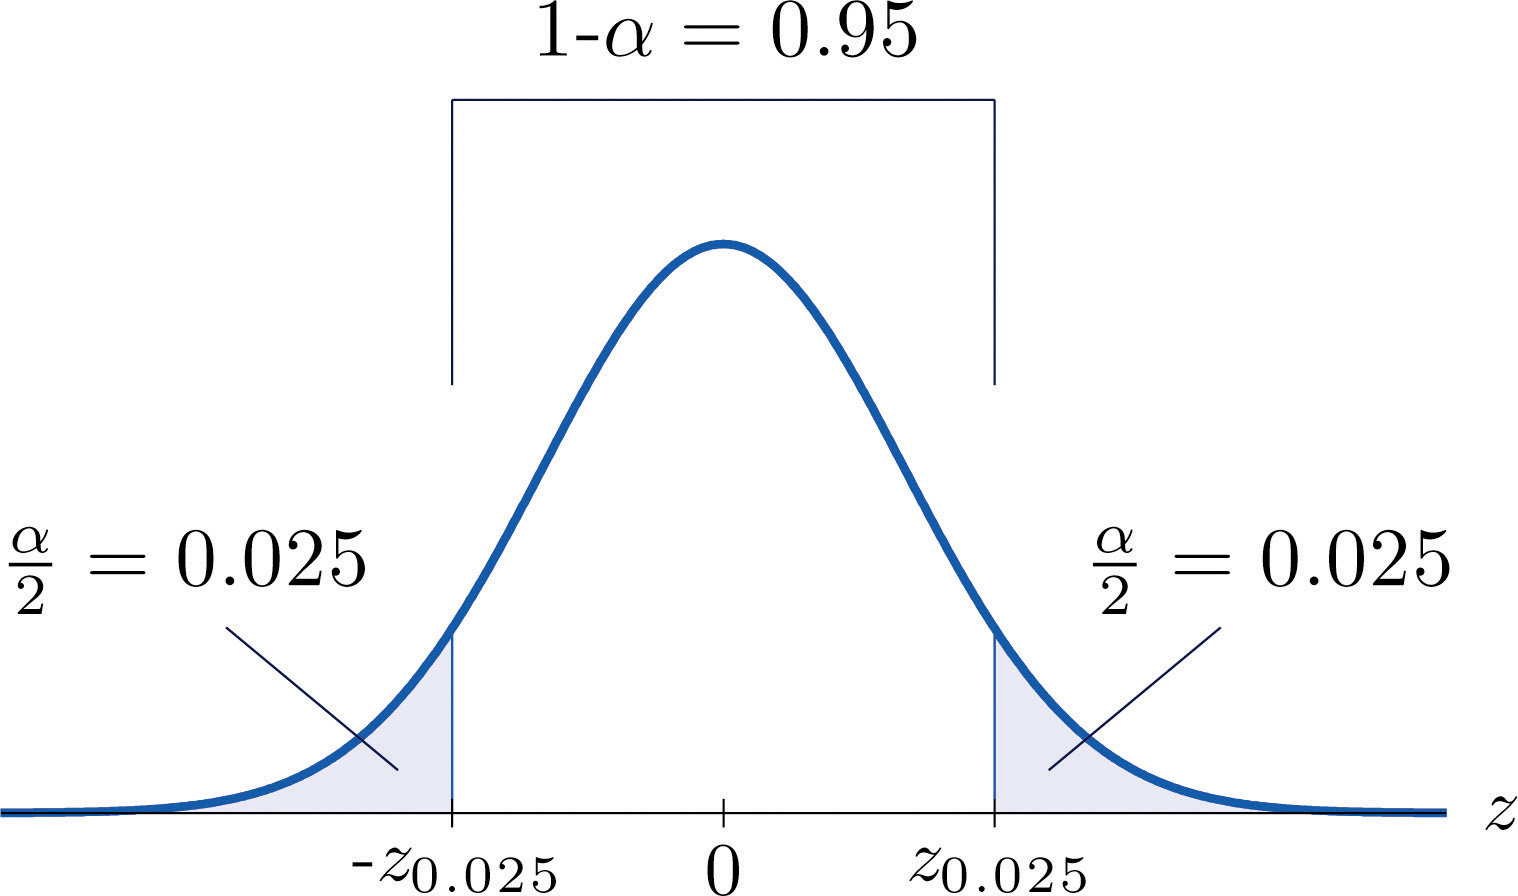
\includegraphics[scale=0.7]{ci_95}
\newline We can see that:
\newline 
\[  P \{ -Z_{\alpha\\/2} \le Z \le Z_{\alpha\\/2}  \}  = 1 - \alpha  \] 
\newline substituting Z into equation:
\[  P \{ -Z_{\alpha\\/2} \le \dfrac{\bar{X} - \mu}{\sigma \\/ \sqrt{n} }  \le Z_{\alpha\\/2}  \}  = 1 - \alpha  \] 
\newline isolating $\mu$:
\[  P \{ \bar{X}-Z_{\alpha\\/2} (\sigma \\/ \sqrt{n}) \le \mu \le \bar{X}+Z_{\alpha\\/2} (\sigma \\/ \sqrt{n})  \}   = 1 - \alpha  \] 
\newline Conclusion
$\left[\bar{X} - Z_{\alpha\\/2} (\sigma \\/ \sqrt{n}), \bar{X} + Z_{\alpha\\/2} (\sigma \\/ \sqrt{n}) \right] $ is a 100(1-$\alpha$) CI for $\mu$ 
\newline
\newline\textbf{How to Construct Confidence Interval Using Pivot Approach:} 
\newline Suppose we have a random sample X$_1$,X$_2$,...,X$_n$ from a population distribution and the parameter of interest is $\theta$.
\newline
\newline Given value $\alpha \in (0,1)$. We would like to construct a 1-$\alpha$ Confidence Interval using a Pivot Approach:
\begin{enumerate}
	\item\textbf{Find a variable Y, that is function of the parameter $\theta$ and data x.}
	\item\textbf{The distribution of newly created variable Y is free of $\theta$.}
\end{enumerate}
\textul{In many cases:}
\newline\Large\rule{3.0cm}{0pt}$Y = \dfrac{\hat{\theta} - \theta}{ SE(\hat{\theta})}$ is a pivot and the distribution of Y is symmetric about 0.
\newline
\newline
\newline\Large\textbf{ Using Pivot Approach for Two-Sided Intervals:}
\newline Find the cut points(quantiles)  c$_{\alpha \\/ 2}$ such that:
\[  P \{ c_{\alpha \\/ 2} \le Y \le c_{\alpha \\/ 2}  \}   = 1 - \alpha  \] 
c$_{\alpha \\/ 2}$ is the upper ($\alpha$ / 2)100th percentile.
%\Large\rule{2.3cm}{0pt} \textbf{fixed}
 %\textbf{(Unbiased Estimator)}\newline
 
\section{}

\end{document}




